\documentclass{sprz}
\usepackage[backend=bibtex,style=numeric,sorting=none]{biblatex}

\addbibresource{bibliography.bib}

\studfield{Informatyka}
\studtype{Zaoczne}
\title{BatMonit -- system wykrywania nietoperzy na farmach wiatrowych}
\engtitle{BatMonit -- bat detection system on wind farms}
\acronym{Batmonit2}
\titledate{2021-11-07}
\supervisor{dr Puźniakowski Tadeusz}
\author{Juliusz Orłowski}{s19799}{Aplikacje Internetowe}{Niestacjonarny}
\author{Jakub Prucnal}{s19800}{Sztuczna Inteligencja}{Niestacjonarny}
\author{Magdalena Wybraniec}{s19798}{Sztuczna Inteligencja}{Niestacjonarny}
\consultant{Dawid Gradolewski}
\consultant{Damian Dziak}
\projectgoals{Projekt typu R\&D, ma na celu wytworzenie systemu softwarowego pobierającego i analizującego dźwięk pochodzący z mikrofonu ultradźwięków oraz rozpoznającego pojawienie się nietoperzy, zapisujący nagrania w bazie danych i wizualizujący je w interfejsie - panelu administratora. Dodatkowo celem będzie przygotowanie analizy odległości i kątów z jakiej mikrofon rejestruje głos nietoperza i adekwatnie – zaproponowanie liczby i rozstawienia urządzeń nasłuchowych, tak aby pokryć kąt 360 stopni wokół turbiny na farmie wiatrowej.}
\productsandservices{System wykrywający nietoperze z nagrań ultradźwięków, możliwy do połączenia z systemem wyłączania turbiny}
\mainfunctionalities{
\begin{itemize}
\item{Mikrofon ultradźwiękowy wraz z oprogramowaniem nagrywającym dźwięk}
\item{Urządzenie do którego nagrania są przesyłane i przechowywane oraz automatycznie analizowane w poszukiwaniu na nim nietoperza}
\item{Baza danych do której trafiają przeanalizowane nagrania}
\item{Interfejs wizualizujący nagrania}
\end{itemize}
}
\successmeasure{Oprogramowanie wykrywające i rozpoznające pojawienie się nietoperzy oraz wytworzenie urządzenia do rejestracji ultradźwięków. Dokonana analiza ulokowania urządzeń rejestrujących na wiatraku oraz jej akceptacja przez konsultanta z firmy BIOSECO.}
\projlimitations{
Czas trwania projektu jest ograniczony do momentu przekazania książki dyplomowej do dziekanatu uczelni PJATK.
Ograniczona dostępność nagrań głosów nietoperzy w full-spectrum – możliwa sytuacja gdy tworzenie projektu będzie odbywało się na podstawie nagrań przetworzonych.
Aktywność nietoperzy ma miejsce od końca marca do października – w związku z tym brak możliwości nagrywania ich aktywności w trakcie semestru zimowego – a tym samym brak możliwości wykonania prób hardware’u przed kwieniem 2022.
}
\date{\today}
\nabstract{TODO}



\begin{document}

\maketitle

\makeprojectcard
\makedeclaration

\tableofcontents

\chapter{Wstęp}\label{ch:wstep}

U podłoża rozwoju alternatywnych źródeł elektryczności leży uczynienie branży energetycznej bardziej „zieloną”, aby życie przyszłych pokoleń było przynajmniej tak samo dobre, jak nasze jest dzisiaj. W poszukiwaniu rozwiązań, które zabezpieczają społeczności w dobie globalnego ocieplenia,  zrównoważony rozwój stał się rdzeniem idei alternatywnych źródeł energii. Druga część historii posiada jednak swą ciemną stronę – wiele danych naukowych wskazuje na znaczący niekorzystny wpływ farm wiatrowych na przyrodę, a zwłaszcza nietoperze. A są one ważnym elementem bioróżnorodności i poszukiwanego zrównoważonego rozwoju. Autorzy pracy dyplomowej w kooperacji z firmą Bioseco wypracowali oparty o sztuczną inteligencję system, który w przypadku dalszego jego rozwijania, zmniejszy śmiertelność nietoperzy na farmach wiatrowych i pomoże utrzymać branży wiatrowej miano ekologicznej. Chiropterologom zaś oraz urzędnikom oceniającym projekty wiatrowe pod kątem realizacji przyrodniczych norm prawnych, zapewni dodatkowe narzędzia minimalizacji wpływu farm na nietoperze.

\section{Cele projektu}

W ramach sformułowanego tematu wyszczególniono następujące cele badawcze i programistyczne:

\begin{itemize}
\item{realizację działającego produktu o minimalnym zestawie funkcjonalności (ang: Minimal Viable Product, dalej: MVP) rejestrującego i identyfikującego nietoperze oraz wysyłającego sygnał wyłączenia – docelowo do systemu turbiny wiatrowej – składającego się z części sprzętowej i oprogramowania: modelu konwolucyjnych sieci neuronowych (ang: convoluted neural network, dalej CNN) oraz z aplikacji użytkownika oraz bazy danych,}
\item{opracowanie koncepcji liczby i układu mikrofonów ultradźwięków docelowego produktu poprzez przeprowadzenie badań terenowych i laboratoryjnych w zakresie zasięgu pracy testowanego sprzętu, tak by cały system pokrywał obszar 360 stopni dookoła turbiny wiatrowej, w odległości do około 100 m,}
\item{opracowanie modelu sieci neuronowych uzyskującego przynajmniej 90\% skuteczności w identyfikacji nietoperzy - borowca wielkiego Nyctalus noctula i karlików Pipistrellus sp., głównych ofiar kolizji z turbinami wiatrowymi,}
\item{przyczynienie się do rozwiązania realnego problemu występującego w obszarze branży energetyki wiatrowej oraz ochrony przyrody,}
\item{rozpoczęcie współpracy z Bioseco Sp. z o.o. w celu zaprezentowania umiejętności studentów firmie oraz ich szybszego rozwijania dzięki kontaktowi z realnymi problemami biznesowymi, merytorycznymi, produkcyjnymi i wdrożeniowymi, rozwiązywanymi aktualnie przed doświadczony zespół specjalistów firmy.}
\end{itemize}

\chapter{Podłoże projektu}

\section{Geneza problemu}

Lądowe farmy wiatrowe mogą mieć znaczący wpływ na środowisko naturalne, w szczególności na nietoperze. Wszystkie gatunki nietoperzy w Polsce są objęte ścisłą ochroną gatunkową i podlegają ochronie prawnej zgodnie z Rozporządzeniem Ministra Środowiska z dnia 16 grudnia 2016 r. w sprawie ochrony gatunkowej zwierząt \cite{Rozporządzenie}. Tym samym inwestor realizujący inwestycję wiatrową przestrzegając prawa ochrony przyrody jest zobligowany uzyskać tzw. Decyzję Środowiskową (dalej: DŚ). Zawarte są w niej wszelkie informacje dotyczące: chiropterofauny danego obszaru, szacowanego wpływu inwestycji na nietoperze, działań zapobiegających i minimalizujących ewentualny wpływ inwestycji na nietoperze, tak by spełniała ona założenia dobrych praktyk i przepisy prawa – polskiego i międzynarodowego. 

Dotychczas przyjętą praktyką w przypadku wykrycia zbyt dużych aktywności nietoperzy w monitoringu przedrealizacyjnym było wpisanie do DŚ obowiązkowych wyłączeń turbin w okresach, w których te zbyt duże aktywności wykryto \cite{Wytyczne}. Jednak dynamika użytkowania przestrzeni przez nietoperze jest bardzo zmienna i po realizacji inwestycji ssaki te mogą mieć bardzo zróżnicowaną aktywność i w całych wyznaczonych okresach nie muszą być zagrożone. A wyłączenia turbin na długie okresy w roku wiążą się z ogromnymi stratami inwestorów. System opracowany w ramach niniejszej pracy inżynierskiej może zapoczątkować nowe standardy na poziomie krajowym, europejskim i światowym, w zakresie niezbędnych działań minimalizujących wpływ siłowni na nietoperze – zamiast dotychczas stosowanych, z góry określonych wyłączeń na długi okres, mogłyby być wykorzystywane wyłączenia sterowane na bieżąco przez system – turbiny zatrzymywane byłyby tylko w czasie, kiedy większe liczebności nietoperzy faktycznie się pojawiają.

\section{Aktualne rozwiązania konkurencyjne}

Intensywny rozwój sieci neuronowych oraz internetu rzeczy (ang: IoT) przyczynił się do powstania podobnych rozwiązań. Na rynku światowym istnieją zbliżone pod kątem funkcjonalnym systemy, takie jak: DTBat i Fleximouse.

\section{IoT}

\section{Sieci neuronowe}

\section{Kooperacja z Bioseco S.A.}

\chapter{Metody pracy}

\section{Proces wytwórczy}

\subsection{Przyjęte podejście}

\subsection{Organizacja zespołu}

\subsection{Charakterystyka przyrostów}

\section{Srodowisko technologiczne}

\subsection{Technologie}

\subsection{Infrastuktura techniczna}

\subsection{Infrastuktura komunikacyjna i dokumentacja}

\section{Analiza zagrożeń}

\chapter{Prace badawczo-rozwojowe i projektowanie}

\section{Konsultacje z Bioseco S.A.}

\section{Konsultacje chiropterologiczne}

\section{Mikrofon ultradźwięków spełniający wymogi końcowego produktu}

\section{Odtwarzanie ultradźwięków}

\section{Głosy nietoperzy typu full-spectrum}

\subsection{Wytworzenie sztucznego głosu nietoperza w programie Audacity}

W celu przetestowania działania sprzętu rejestrującego i oprogramowania przetwarzającego zarejestrowane dźwięki, przeprowadzono doświadczenie polegające na sztucznym wytworzeniu dźwięków, które imitowały by głos nietoperza.
Pierwszym etapem było wygenerowanie w programie Audacity sinusoidalnej fali dźwiękowej z początkową częstotliwością 51 kHz i końcową częstotliwością 42 kHz, amplitudą początkową 0 i amplitudą końcową 1, interpolacją logarytmiczną oraz czasem trwania 25 ms (\ref{img:wykres_fali}).

\begin{figure}[h]
    \centering
    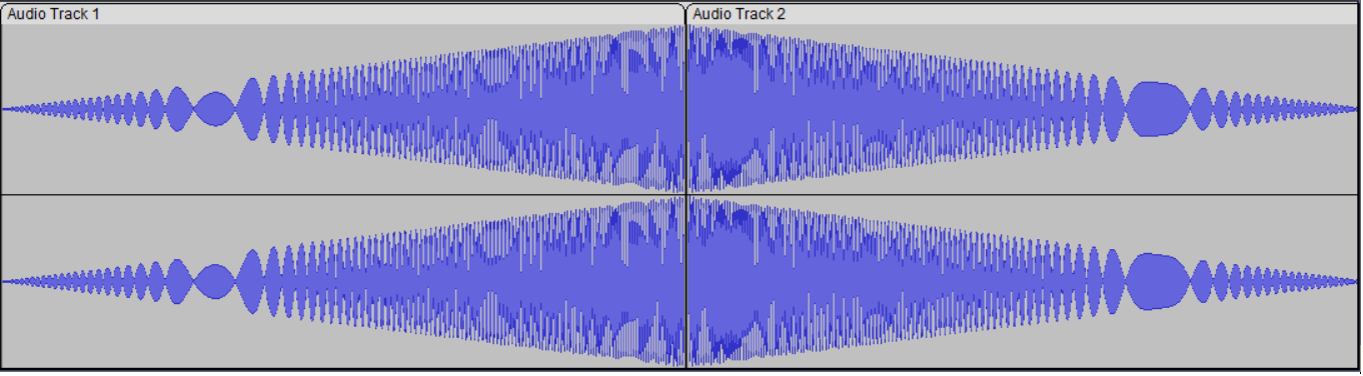
\includegraphics[width=0.8\textwidth]{sprz/wykres_fali}
    \caption{Wykres fali dźwiękowej}
    \label{img:wykres_fali}
\end{figure}

Uzyskany w ten sposób wykres fali dźwiękowej skopiowano dziesięciokrotnie i utworzono sekwencję 500 ms dźwięków, przed którą i po której wprowadzono 500 ms ciszy w celu łatwiejszego wyodrębnienia dźwięków po ich późniejszym zarejestrowaniu (\ref{img:wykres_fali_wielokrotnej}).

\begin{figure}[h]
    \centering
    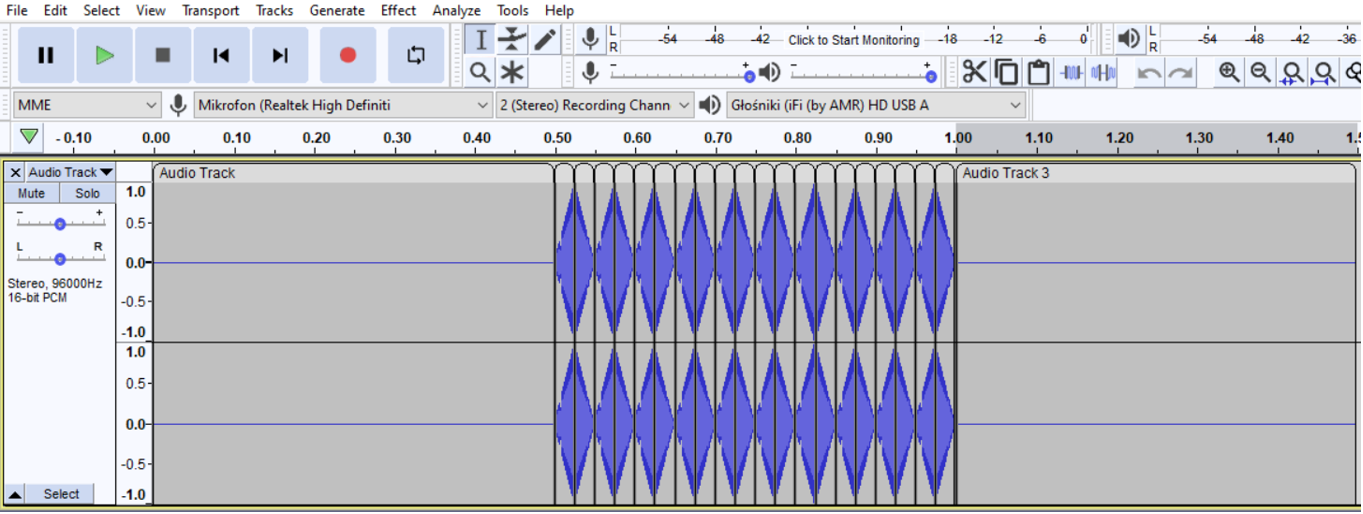
\includegraphics[width=0.8\textwidth]{sprz/wykres_fali_wielokrotnej}
    \caption{Zwielokrotniony wykres fali}
    \label{img:wykres_fali_wielokrotnej}
\end{figure}

Następnie, do wyemitowania dźwięku doświadczenia niezbędne były urządzenia obsługujące co najmniej dwukrotnie wyższą częstotliwość niż emitowane dźwięki. W tym celu do komputera służącego jako generator dźwięku podłączono wzmacniacz iFi Zen Dac o maksymalnej częstotliwości odtwarzania 384 kHz oraz głośnik ultradźwiękowy Pettersson L400 (10-110 kHz). Do zarejestrowania wyemitowanego dźwięku posłużył mikrofon Pettersson M500-384 o częstotliwości próbkowania 384 kHz.

Program BatSound dołączony do mikrofonu posłużył do wizualizacji zarejestrowanego dźwięku.

\begin{figure}[h]
    \centering
    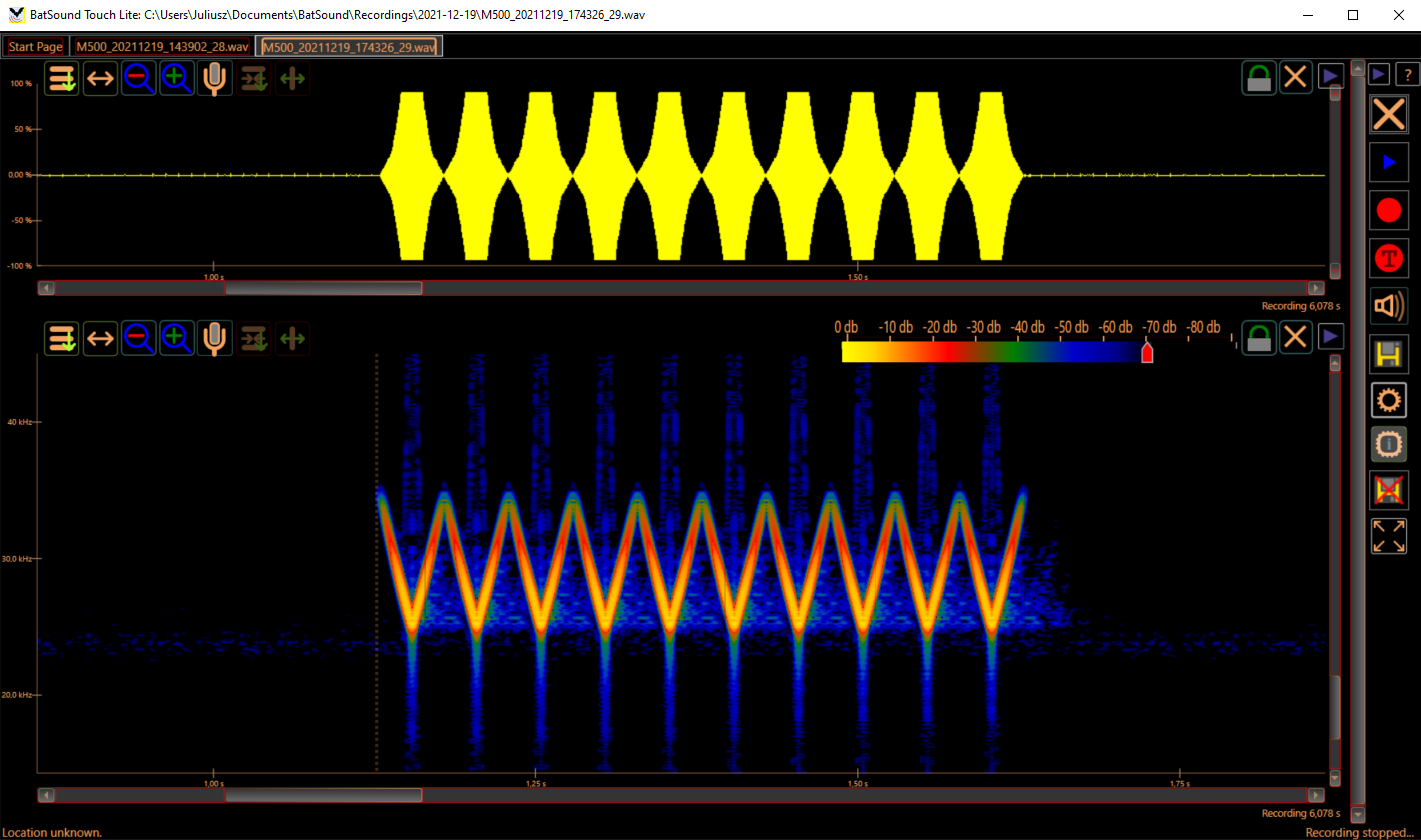
\includegraphics[width=0.8\textwidth]{sprz/batsound}
    \caption{Wykres zarejestrowanego dźwięku zwizualizowany w programie Batsound}
    \label{img:batsound}
\end{figure}

Powyższe doświadczenie dowiodło, iż mikrofon Pettersson M500-384 spełnia swoje zadanie. Mikrofon rejestruje dźwięki w zakresie niesłyszalnym dla człowieka i poprawnie wizualizuje zarejestrowane nagranie.

\subsection{Zebranie nagrań nietoperzy}

\chapter{Struktura produktu}

Struktura wytworzonego produktu została przedstawiona w podziale na poszczególne komponenty.

\section{Architektura systemu}

Na poniższych modelach przedstawiono najważniejsze elementy logiczne, urządzenia wejścia-wyjścia oraz obieg informacji w systemie (\ref{img:model_architektury}). W celu ułatwienia zrozumienia osadzenia systemu w rzeczywistości, architekturę zobrazowano również w postaci graficznej, łącznie z widokiem interfejsu (\ref{img:reprezentacja_graficzna}). 

\begin{figure}[h]
    \centering
    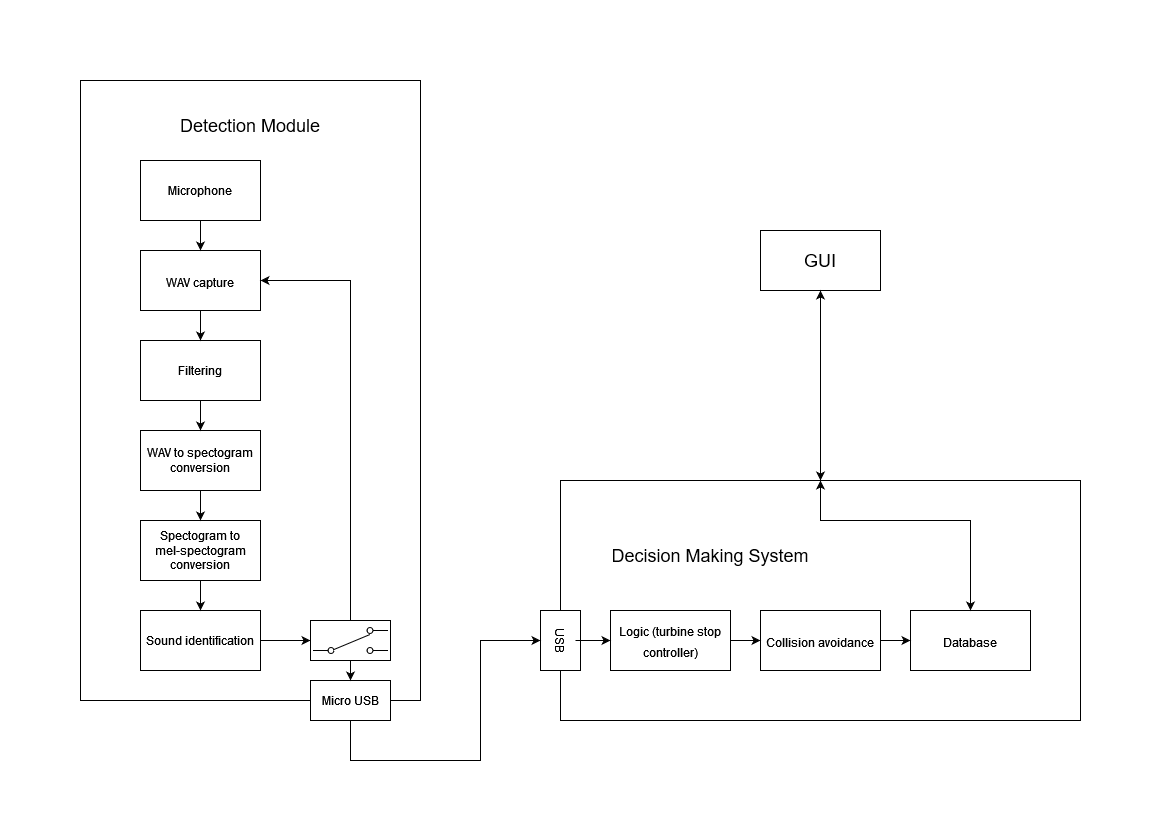
\includegraphics[width=0.8\textwidth]{sprz/model_architektury}
    \caption{Logiczny model architektury systemu}
    \label{img:model_architektury}
\end{figure}

\begin{figure}[h]
    \centering
    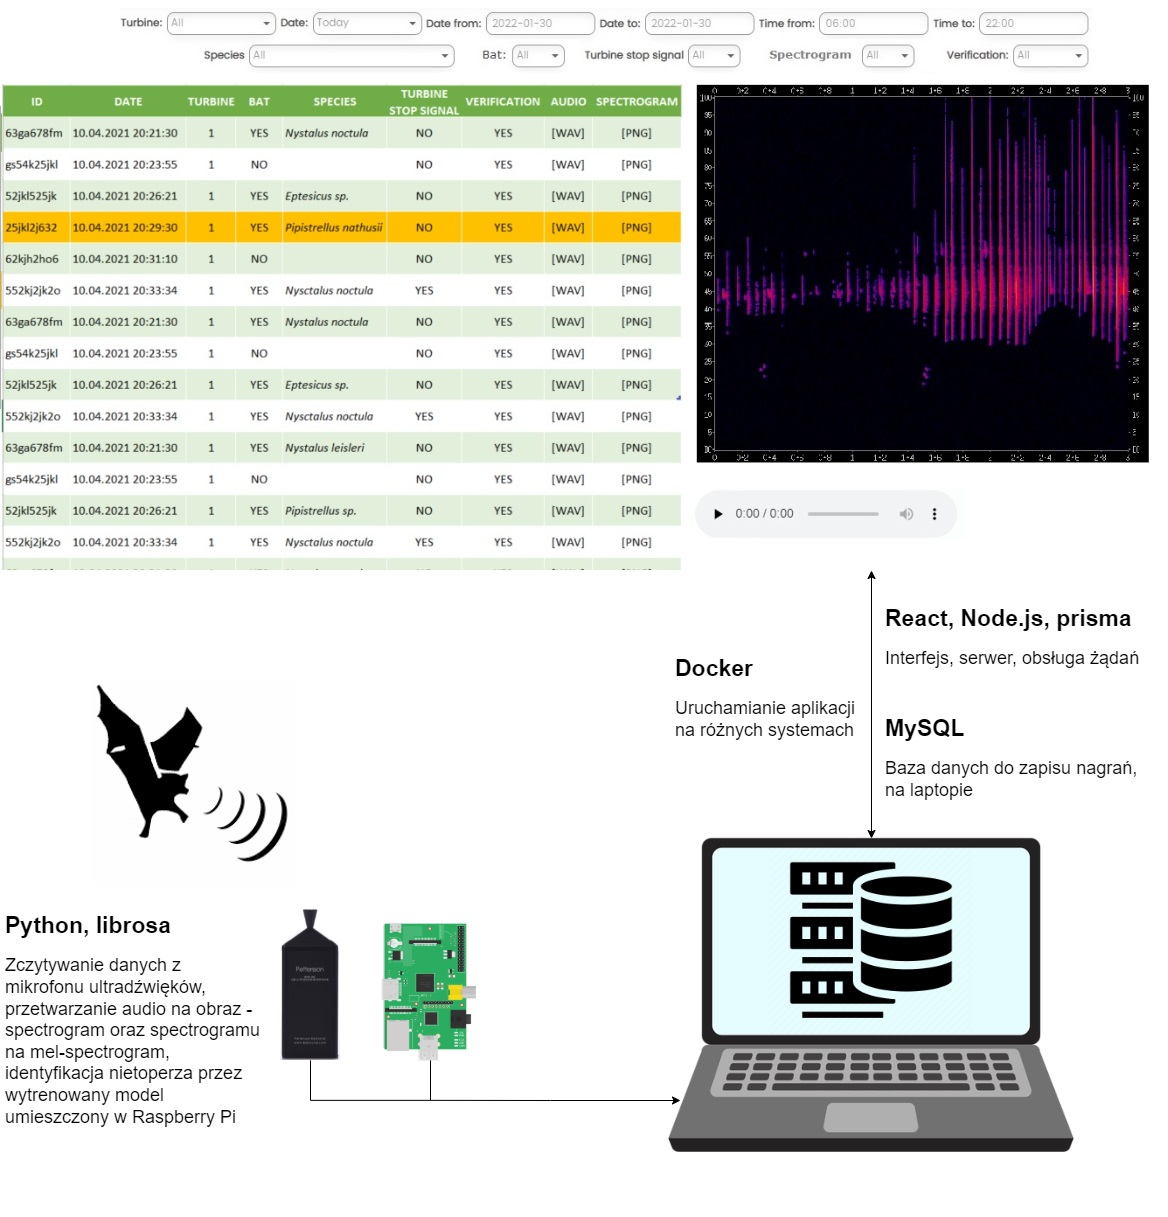
\includegraphics[width=0.8\textwidth]{sprz/reprezentacja_graficzna}
    \caption{Logiczny model architektury systemu}
    \label{img:reprezentacja_graficzna}
\end{figure}

\section{Hardware}

\section{Platforma pobierająca i przetwarzająca nagrania z mikrofonu ultradźwięków}

\section{Model sieci neuronowej}

\section{Baza danych}

\section{Aplikacja użytkownika}

\chapter{Realizacja sieci neuronowej}

\section{Przygotowanie danych}

\subsection{Czyszczenie}

\subsection{Dobór typu spektogramu}

\subsection{Cięcie}

\subsection{Augmentacja}

\section{Dobór sieci neuronowej}

\subsection{Przegląd literatury}

\subsection{Konsultacje}

\section{Dobór parametrów sieci neuronowej}

\subsection{Funkcje aktywacji}

\subsection{Funkcja błędu}

\subsection{Optymalizatory}

\subsection{Regularyzacja}

\subsection{Parametry warstw sieci}

\subsection{Transfer learning}

\section{Skuteczność sieci neuronowej}

\subsection{Macierz pomyłek}

\subsection{Metryki}

\subsection{Learning rate}

\chapter{Realizacja interfejsu użytkownika i bazy danych}

\section{Implementacja interfejsu użytkownika}

\section{Implementacja bazy danych}

\chapter{Testowanie}

\section{Testy terenowe produktu}

\section{Testy oprogramowania}

\subsection{Testy jednostkowe}

\subsection{Testy integracyjne}

\subsection{Testy funkcjonalne}

\subsection{Testy akceptacyjne}

\chapter{Przyszłość produktu i komercjalizacja}

\chapter{Podsumowanie}

\chapter{Wkład własny}

\section{Juliusz Orłowski}

\subsection{Wytworzenie sztucznego głosu nietoperza}

\subsection{Interfejs użytkownika}

\subsection{Baza danych}

\subsection{Książka projektu}

\section{Jakub Prucnal}

\subsection{Interfejs użytkownika}

\subsection{Baza danych}

\subsection{Przygotowanie danych do modelu}

\subsection{Model sieci neuronowej}

\subsection{Książka projektu}

\section{Magdalena Wybraniec}

\subsection{Zebranie nagrań nietoperzy}

\subsection{Interfejs użytkownika}

\subsection{Baza danych}

\subsection{Konsultacje chiropterologiczne}

\subsection{Przygotowanie danych do modelu}

\subsection{Model sieci neuronowej}

\subsection{Książka projektu}

\chapter{Załączniki}

\section{Dokument założeń wstępnych}

\section{Specyfikacja wymagań systemowych}

\section{Diagram przypadków użycia}

\chapter{Karty udziałowca}


\begin{stakeholder}[label={tab:stakeholder:someholder},caption={Przykładowy opis udzialowca}]
    \id{jednoznaczny symbol np. UOB 01, UOB 02 ... dla udziałowców ożywionych bezpośrednich, UNP 01... dla nieożywionych pośrednich itd.}
    \name{nazwa udziałowca}
    \descr{opis udziałowca}
    \type{ożywiony/nieożywiony, bezpośredni/pośredni}
    \viewpoint{z jakiej perspektywy patrzy udziałowiec np. technicznej, ekonomicznej, operatora systemu itp.}
    \limitations{ograniczenia udziałowca np. administrator nie powinien specyfikować wymagań finansowych}
    \requ{tu tylko symbole wymagań wyspecyfikowanych w rozdziale 3}
\end{stakeholder}

\chapter{Wymagania wszelakie}

Na tabeli \ref{tab:requirements:general} pokazano jak można definiować wymagania ogólne lub dziedzinowe.

\begin{requirementstab}[label={tab:requirements:general},caption={Przykładowe wymaganie ogólne lub dziedzinowe}]
    \id{jednoznaczny symbol np. WO1, WO2 .. }
    \priority{ważność wymagania, np. wg skali MoSCoW: M – must (musi być) S – should (powinno być) C – could (może być) W – won't (nie będzie – nie będzie implementowane w danym wydaniu, ale może być rozpatrzone w przyszłości )}
    \name{krótki opis}
    \descr{opis szczegółowy, należy dążyć do tego, żeby wszystkie znane na ten moment szczegóły wymagania zostały wydobyte i wyspecyfikowane}
    \sholder{nazwa udziałowca, który podał wymaganie}
    \reqrelated{wymagania zależne i uszczegóławiające – odesłanie poprzez identyfikator}
\end{requirementstab}

Teraz czas na wymagania funkcjonalne, na przykład \ref{tab:requirements:func1}

\begin{requirementstab}[label={tab:requirements:func1},caption={Pryzkładowa tabela z wymaganiami na interfejs z otoczeniem}]
    \id{jednoznaczny symbol np. FO1, FO2 .. }
    \priority{ważność wymagania, np. wg skali MoSCoW: M – must (musi być) S – should (powinno być) C – could (może być) W – won't (nie będzie – nie będzie implementowane w danym wydaniu, ale może być rozpatrzone w przyszłości )}
    \name{krótki opis}
    \descr{opis szczegółowy, należy dążyć do tego, żeby wszystkie znane na ten moment szczegóły wymagania zostały wydobyte i wyspecyfikowane

    Można zastosować opis jak w User Story
    \begin{itemize}
        \item Jako.. (konkretny użytkownik systemu)
        \item chcę... (pożądana cecha lub problem, który trzeba rozwiązać)
        \item bo wtedy/ponieważ… (korzyść płynąca z ukończenia story)
    \end{itemize}
    }
    \acceptcrit{Warunki Satysfakcji (Szczegóły dodane na potrzeby  testów akceptacyjnych)}
    \inputdata{uzupełniane w trakcie sprintu – dane wejściowe, związane z wymaganiem}
    \preconditions{ uzupełniane w trakcie sprintu – warunki, które muszą być prawdziwe przed wywołaniem operacji}
    \postconditions{ uzupełniane w trakcie sprintu – warunki, które muszą być prawdziwe po wywołaniu operacji}
    \exceptions{ uzupełniane w trakcie sprintu – niepożądane sytuacje i sposoby ich obsługi}
    \implementation{ uzupełniane w trakcie sprintu – opis sposobu realizacji}
    \sholder{nazwa udziałowca, który podał wymaganie}
    \reqrelated{wymagania zależne i uszczegóławiające – odesłanie poprzez identyfikator}
\end{requirementstab}


Natomiast tabela \ref{tab:requirements:env1} pokazuje wymagania na interfejs z otoczeniem.

\begin{requirementstab}[label={tab:requirements:env1},caption={Pryzkładowa tabela z wymaganiami na interfejs z otoczeniem}]
    \id{jednoznaczny symbol np. IO1, IO2 .. }
    \priority{ważność wymagania, np. wg skali MoSCoW: M – must (musi być) S – should (powinno być) C – could (może być) W – won't (nie będzie – nie będzie implementowane w danym wydaniu, ale może być rozpatrzone w przyszłości )}
    \name{krótki opis}
    \descr{opis szczegółowy, należy dążyć do tego, żeby wszystkie znane na ten moment szczegóły wymagania zostały wydobyte i wyspecyfikowane}
    \acceptcrit{Warunki Satysfakcji (Szczegóły dodane na potrzeby  testów akceptacyjnych)}
    \inputdata{uzupełniane w trakcie sprintu – dane wejściowe, związane z wymaganiem}
    \preconditions{ uzupełniane w trakcie sprintu – warunki, które muszą być prawdziwe przed wywołaniem operacji}
    \postconditions{ uzupełniane w trakcie sprintu – warunki, które muszą być prawdziwe po wywołaniu operacji}
    \exceptions{ uzupełniane w trakcie sprintu – niepożądane sytuacje i sposoby ich obsługi}
    \implementation{ uzupełniane w trakcie sprintu – opis sposobu realizacji}
    \sholder{nazwa udziałowca, który podał wymaganie}
    \reqrelated{wymagania zależne i uszczegóławiające – odesłanie poprzez identyfikator}
\end{requirementstab}

Tabela dotycząca wymagań pozafunkcjonalnych \ref{tab:requirements:nonfunc1} jest także widoczne.

\begin{requirementstab}[label={tab:requirements:nonfunc1},caption={Pryzkładowa tabela z wymaganiami pozafunkcjonalnymi}]
    \id{jednoznaczny symbol np. NFO1, NFO2 .. }
    \priority{ważność wymagania, np. wg skali MoSCoW: M – must (musi być) S – should (powinno być) C – could (może być) W – won't (nie będzie – nie będzie implementowane w danym wydaniu, ale może być rozpatrzone w przyszłości )}
    \name{krótki opis}
    \descr{opis szczegółowy, należy dążyć do tego, żeby wszystkie znane na ten moment szczegóły wymagania zostały wydobyte i wyspecyfikowane}
    \acceptcrit{Warunki Satysfakcji (Szczegóły dodane na potrzeby  testów akceptacyjnych)}
    \sholder{nazwa udziałowca, który podał wymaganie}
    \reqrelated{wymagania zależne i uszczegóławiające – odesłanie poprzez identyfikator}
\end{requirementstab}


\printbibliography[title={Bibliografia}, heading=bibintoc]




\end{document}
